\documentclass{article}

% Language setting
% Replace `english' with e.g. `spanish' to change the document language
\usepackage[english,russian]{babel}
\usepackage{amsmath}

%графика
\usepackage{wrapfig}
\usepackage{graphicx}
\usepackage{pgfplots}
\usepackage{tikz}
\usepackage{svg}

\usepackage{tcolorbox}

% Set page size and margins
% Replace `letterpaper' with `a4paper' for UK/EU standard size
\usepackage[letterpaper,top=2cm,bottom=2cm,left=3cm,right=3cm,marginparwidth=1.75cm]{geometry}

% Useful packages
\usepackage{amsmath}
\usepackage{amssymb}
\usepackage{graphicx}
\usepackage{fixltx2e}
\usepackage[colorlinks=true, allcolors=blue]{hyperref}

\usepackage{geometry}
\geometry{left=25mm,right=25mm,
 top=25mm,bottom=25mm}

\usepackage[dvipsnames]{xcolor} % for RoyalBlue
\usepackage{hyperref}
\hypersetup{colorlinks=true, linkcolor=blue, urlcolor=blue, citecolor=blue}  


\title{Количественная аналитика\\
Лекции (1 -- 2 неделя) \\
Что особенно важно знать о случайных процессах
}
\author{Максим Соснин}

% Колонтитулы
\usepackage{fancyhdr}
\pagestyle{fancy}
\renewcommand{\headrulewidth}{0.1mm}  
\renewcommand{\footrulewidth}{0.1mm}
\lfoot{}
\rfoot{\thepage}
\cfoot{}
\rhead{CMF-2022}
\chead{}

\begin{document}
\maketitle

% Оглавление
\setcounter{tocdepth}{2} % {2} - в оглавлении участвуют chapter, section и subsection. {1} - только chapter и section
\renewcommand\contentsname{Содержание}
\tableofcontents
\newpage

% \section{Dictionary, Definitions, Abbreviations}

% \subsection{Dictionary}
% \begin{itemize}
%     \item IR - Interest rate - процентная ставка.
%     \item Compounding - платежи (idk)
% \end{itemize}

% \subsection{Definitions and Abbreviations}
% \begin{itemize}
%     \item SAR - Stated annual rate.
%     \item EAR - Effective annual rate.
%     \item FoC - Frequency of Compounding
%     \item PMT - Payment
%     \item r - Interest rate (at the moment). 
% \end{itemize}

\newcommand{\E}{\textrm{E}}
% equation sign with annotation above it
\newcommand\eqannot[1]{\stackrel{\mathclap{\normalfont\mbox{#1}}}{=}}

\section{Случайный процесс}
\subsection{Определение}
\begin{itemize}
    \item{
        \textbf{Дискретный случайный процесс} -- это набор случайных величин $\{X_{t_1}, X_{t_2}, ..., X_{t_n}\}$, индексированных некоторым параметром $t \in \{t_1, t_2, ..., t_n\}$. 

        Параметр $t$ может быть временем, тогда $t_i$ -- это моменты времени, в которые была зарегистрирована случайная величина. Однако параметр может иметь и другие значения, например, координата. Далее будем подразумевать, что параметр -- это время.

        Распределения случайных величин $X_{t_i}$ могут быть как одинаковыми, так и разными.
    }

    \item{
        \textbf{Непрерывный случайный процесс} -- это случайный процесс, параметр которого изменяется непрерывно. Обозначение: $\xi_t$ или $\xi(t)$, где $t$, к примеру, принимает значения из отрезка $[0, T]$.
    } 
\end{itemize}

\subsection{Характеристики случайного процесса}
\begin{itemize}
    \item{
        \textbf{Среднее значение}
        $$\textrm{E}[X_{t_i}] = \mu(t_i)$$
        $$\textrm{E}[\xi_t] = \mu(t)$$
        
        Среднее значение случайного процесса в общем случае зависит от времени.
    }

    \item{
        \textbf{Дисперсия}

        $$
        \textrm{D}[\xi_t] \equiv 
        \textrm{Var}[\xi_t] = 
        %\textrm{E}[(\xi_t - \textrm{E}[\xi_t])^2] =
        \textrm{E}[\xi_t^2] - \textrm{E}[\xi_t]^2 =
        \sigma^2(t)
        $$
        
        Дисперсия случайного процесса в общем случае также зависит от времени.
    }

    \item{
        \textbf{Ковариация (autocovariance, covariance)}

        $$\textrm{cov}(\xi_t, \xi_s) = \textrm{E}[(\xi_t - \mu(t))(\xi_s - \mu(s))]$$

        \textit{В англоязычной литературе данная характеристика случайного процесса называется \\\textbf{autocovariance}, поскольку это ковариация случайного процесса с самим собой в различные пары моментов времени. Существует путаница между русскоязычной и англоязычной терминологией, связанной с ковариацией и корреляцией. См. \href{https://en.wikipedia.org/wiki/Autocovariance}{https://en.wikipedia.org/wiki/Autocovariance},\\ \href{https://en.wikipedia.org/wiki/Autocorrelation}{https://en.wikipedia.org/wiki/Autocorrelation}
        }.
    }

    \item{
        \textbf{Корреляция (autocorrelation, correlation)}
        % \textrm{cov}
        $$\textrm{corr}(\xi_t, \xi_s) = \frac{\textrm{cov}(\xi_t, \xi_s)}{\sqrt{\sigma_{\xi}^2(t) \cdot \sigma_{\xi}^2(s)}} $$
    }

    \item{\textbf{Моменты} -- начальный, центральный, смешанный, ...}
\end{itemize}

\subsection{Стационарный случайный процесс}
Случайный процесс называется \textbf{стационарным}, если его среднее значение и дисперсия (а следовательно, и все последующие моменты) не зависят от времени.

$$\textrm{E}[\xi_t] = \mu = const$$
$$\textrm{D}[\xi_t] = \sigma^2 = const$$
Различают стационарность \textbf{в узком смысле} и стационарность \textbf{в широком смысле}.

\section{Случайное блуждание}
\subsection{Определение}
Рассмотрим сумму независимых и одинаково распределённых случайных величин в моменты времени $t_k$:

$$S_n = \sum_{k=1}^n X_{t_k}, \quad \forall i \, X_{t_i} - \textrm{i.i.d.} $$
Ряд $\{S_n\}$ называется \textbf{случайным блужданием}.

\noindent
Случайное блуждание также можно определить следующим образом:
$$S_n = S_{n-1} + X_{t_n}$$

\subsection{Среднее значение и дисперсия} \label{ssec:random-walk-mean-variance}
\begin{itemize}
    \item{
        Среднее значение случайного блуждания:
        $$\E[S_n] = \sum_{k=1}^n \E[X_{t_k}] = \sum_{k=1}^n \mu = n \mu,$$
        где $\mu = \E[X_{t_i}]$.
    }
    \item{
        Дисперсия случайного блуждания:
        $$
        \textrm{D}[S_n] = 
        \textrm{D}\left[\sum_{k=1}^n X_{t_k} \right] =
        \sum_{k=1}^n \textrm{D}[X_{t_k}] = 
        n \sigma^2,
        $$ 
        где $\sigma^2 = \textrm{D}[X_{t_i}]$. (Здесь дисперсия суммы равна сумме дисперсий, потому что $X_{t_i}$ -- независимы и одинаково распределены.)
    }
\end{itemize}

\subsection{Отнормированное случайное блуждание}
Осуществим нормировку случайных величин $X_{t_i}$:
$$Y_{t_i} = \frac{X_{t_i} - \mu}{\sigma}.$$
Получим новое случайное блуждание
$$\widetilde S_n = \sum_{k=0}^n Y_{t_k}$$
со средним значением $\E[\widetilde S_n] = 0$ и дисперсией $\textrm{D}[\widetilde S_n] = n$.

\section{Винеровский процесс}
\subsection{Винеровский процесс как предельный случай случайного блуждания}
Винеровский процесс можно определить как предельный случай случайного блуждания. Разобьём отрезок $[0, t]$ точками $0 = t_0 < t_1 < t_2 < ... < t_{N-1} < t_N = t$ на $N$ равных отрезков длины $\Delta t = t / N$. 

\begin{figure}[h]
\centering
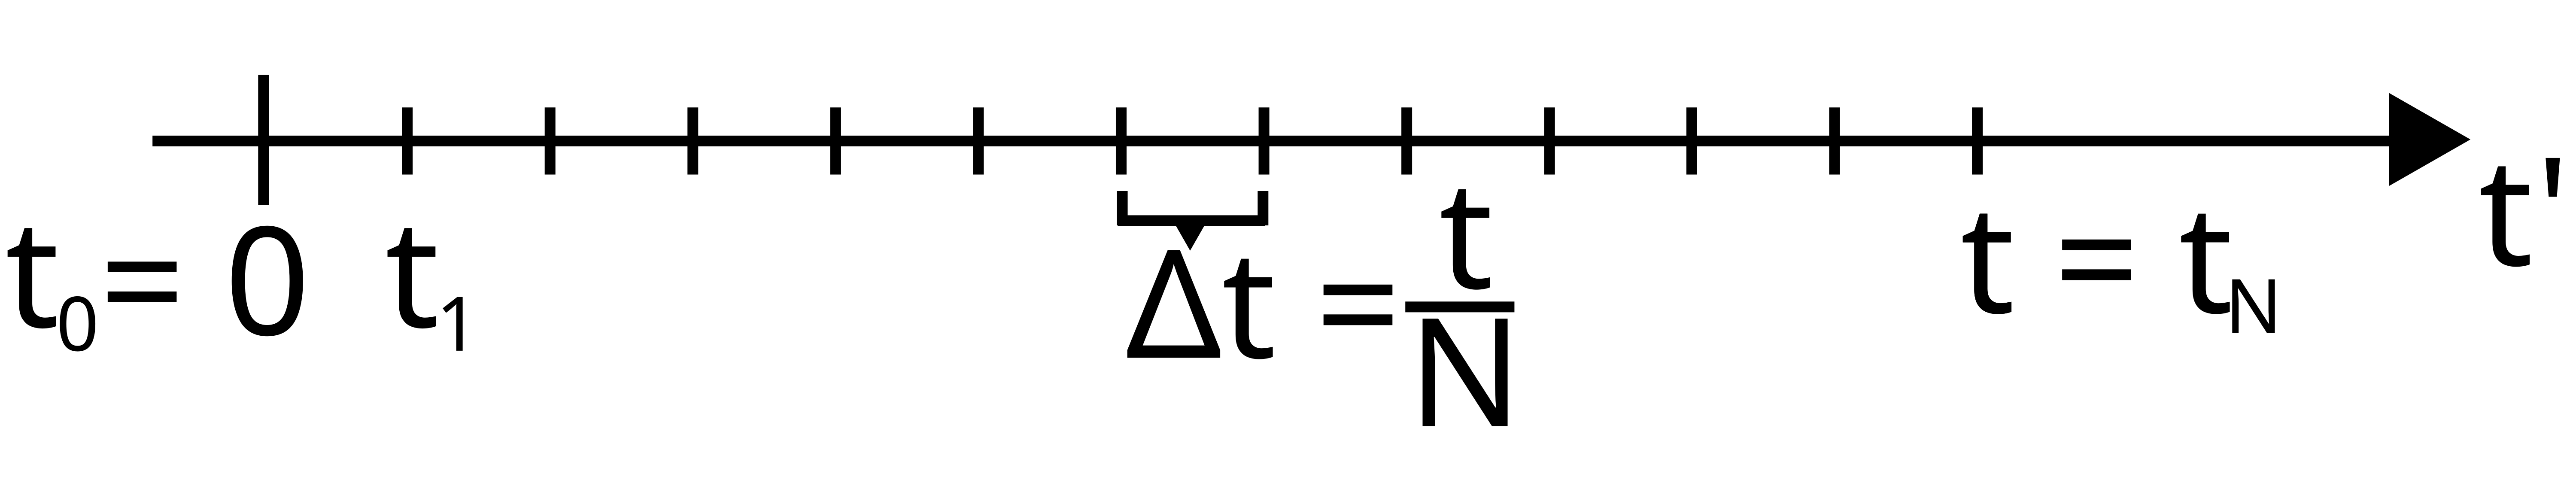
\includegraphics[width=0.45\textwidth]{number-line.png}
%\caption{Разбиение отрезка}
\label{number-line}
\end{figure}

\noindent
Пусть $\varepsilon_i,\ i \in [0..N]$ -- независимые и одинаково распределенные случайные величины со средним значением $0$ и дисперсией $1$. Каждой точке $t_i$ поставим в соответствие случайную величину $\varepsilon_i$.

Рассмотрим случайное блуждание
$$ \widetilde W_t = \sum_{k=0}^N \varepsilon_k \cdot (\Delta t)^\alpha,$$
где $\alpha$ -- некоторое число, которое мы пока что не знаем. Заметим, что случайная величина $\varepsilon_k \cdot (\Delta t)^\alpha$ имеет среднее значение $0$ и стандартное отклонение $(\Delta t)^\alpha$. Случайное блуждание $W_t$ будет иметь следующие значения среднего и дисперсии (см. пункт \ref{ssec:random-walk-mean-variance}):
$$\E[\widetilde W_t] = 0,$$
$$
\textrm{D}[\widetilde W_t] =
N (\Delta t)^{2\alpha} =
N \left( \frac{t}{N} \right)^{2\alpha} =
\frac{t^{2\alpha}}{N^{2\alpha-1}}.
$$
Если мы устремим $N$ к $\infty$, то при $\alpha > \frac{1}{2}$, $\textrm{D}[\widetilde W_t] \to 0$, а при $\alpha < \frac{1}{2}$, $\textrm{D}[\widetilde W_t] \to \infty$. Поэтому единственно возможное значение $\alpha = \frac{1}{2}$ (\textit{лектор не поясняет, почему так}), при котором $\textrm{D}[\widetilde W_t] = t$. Таким образом, при $N\to\infty$, мы получаем непрерывный случайный процесс со средним $0$ и дисперсией $t$, который называется \textbf{винеровским процессом}:
$$
W_t =
\lim_{N\to\infty} \widetilde W_t =
\lim_{N\to\infty} \sum_{k=0}^N \varepsilon_k \cdot \sqrt{\Delta t} =
\sqrt{t} \lim_{N\to\infty} \frac{1}{\sqrt{N}} \sum_{k=0}^N \varepsilon_k \eqannot{ЦПТ}
\sqrt{t} \cdot N(0, 1),
$$
где $N(0, 1)$ -- стандартное нормальное распределение. В последнем равенстве переход совершён благодаря центральной предельной теореме.

Отметим, что винеровский процесс не является стационарным, поскольку $\textrm{D}[W_t] = t$.

Также отметим, что ковариация винеровского процесса
$$\textrm{cov}(W_t, W_s) = \min(t, s)$$
(см. \href{https://en.wikipedia.org/wiki/Wiener_process#Covariance_and_correlation}{https://en.wikipedia.org/wiki/Wiener\_process\#Covariance\_and\_correlation}).


\subsection{Примеры винеровских процессов}
\begin{itemize}
    \item{
        \textbf{Стандартизированный винеровский процесс}
        $$W_t = \sqrt{t} \cdot N(0, 1)$$
    }
    \item{
        \textbf{Не стандартизированный винеровский процесс}
        $$W_t = \sigma \sqrt{t} \cdot N(0, 1),$$
        где $\sigma$ -- некоторое положительное число.
    }
    \item{
        \textbf{Винеровский процесс со сдвигом (with drift)}
        $$Y_t = \mu t + \sigma W_t,$$
        где $\mu$ и $\sigma$ -- некоторые числа ($\sigma > 0$). При этом $\E[Y_t] = \mu t$.
    }
\end{itemize}


\end{document}
